\documentclass[conference]{IEEEtran}
\usepackage{cite}
\usepackage{amsmath,amssymb,amsfonts}
\usepackage{algorithmic}
\usepackage{graphicx}
\usepackage{textcomp}
\usepackage{xcolor}
\def\BibTeX{{\rm B\kern-.05em{\sc i\kern-.025em b}\kern-.08em
    T\kern-.1667em\lower.7ex\hbox{E}\kern-.125emX}}
\begin{document}

\title{Multicasting in Wavelength Division Multiplexing (WDM) networks and EONs}

\author{\IEEEauthorblockN{Agnieszka Musiał}
\IEEEauthorblockA{\textit{Politechnika Wrocławska} \\
\textit{Wydział Informatyki i Telekomunikacji} \\
Wrocław, Poland \\
200910@student.pwr.edu.pl}
\and
\IEEEauthorblockN{André Carvalho}
\IEEEauthorblockA{\textit{University of Aveiro} \\
\textit{Department of Electronics, Telecommunication and Informatics}\\
Aveiro, Portugal \\
andrebcarvalho@ua.pt}
}

\maketitle

\begin{abstract}
This paper provides a literature review of multicast routing in Wavelength Division Multiplexing (WDM) networks and Elastic Optical Networks (EONs). There is a need for effective solutions in computer networks due to the immense and accelerating growth of Internet traffic. WDM technology and EONs are known to increase bandwidth capacity and can be part of the solution.
\end{abstract}

\begin{IEEEkeywords}
elastic optical networks, wavelength division multiplexing, routing, multicasting
\end{IEEEkeywords}

\section{Introduction}

\subsection{Multicasting}
Multicasting is a type of routing scheme in a network where data is transferred from the root node to selected receiving nodes.

In multicast data is propagated over minimum Steiner tree or minimum spanning tree of all recipients so that it is sent over each link exactly once \cite{multicast_definition}. It is more efficient than unicasting to selected nodes. Even though unicast also adopts a minimum Steiner tree or minimum spanning tree, paths are calculated separately between the root and each receiving node. Data would likely be sent over the same link multiple times if that link exists in many calculated paths.

Therefore multicast requires less traffic than unicast.

\subsection{Wavelength division multiplexing}
Wavelength division multiplexing (WDM) is physical technology that increases the capacity of optical fibre by using electromagnetic properties of light.

In fibre-optic communication carrier of data is light. Essentially it is an electromagnetic wave with inversely proportional properties of wavelength and frequency. Light of different wavelengths can be multiplexed together, creating a complex signal that can be transferred over a single optical fibre\cite{wdm_general}. At the receiving end signal is demultiplexed back into many signals, and each is provided to corresponding recipients.

Following are types of WDM systems \cite{cwdm} \cite{dwdm}:
\begin{itemize}
	\item normal (WDM), wavelengths 1310 nm and 1550 nm on one fibre
	\item coarse (CWDM), wavelengths 1271 nm to 1611 nm with channel spacing 20 nm
	\item dense (DWDM), wavelengths 1530 nm to 1565 nm with channel spacing 0.8/0.4 nm
\end{itemize}

A substantial component of WDM is thin-film filters. They can pass certain wavelengths and reflect all other wavelengths; WDM demultiplexer uses this characteristic. Thin-film filters form a cascade, efficiently extracting original signals. Figure \ref{demultiplexing} presents an exemplary design of such a system.

\begin{figure}[htbp]
	\centerline{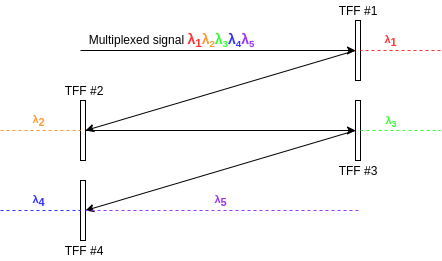
\includegraphics[scale=0.5]{demultiplexer.png}}
	\caption{Demultiplexing in WDM}
	\label{demultiplexing}
\end{figure}

\subsection{Elastic optical networks}
The idea for an elastic optical network (EON) stems from WDM systems. Mikavica \& Kostić-Ljubisavljević, 2020 \cite{eon_definition} define it as:

\begin{quote}
Optical network architecture providing data transmission with spectrum allocation depending on traffic demands.
\end{quote}

WDM network is rigid in resource distribution. It imposes complete allocation of one wavelength, even if the amount of data transferred is far below channel capacity. Algorithms, which optimize resource allocation, improve that, but true innovation lies in EON and its finer granularity of available spectrum resources.

EON introduces slithering of optical spectrum into frequency slots (FS), which are 25, 12.5 or 6.25 GHz wide \cite{eon_fs}. A couple of FS construct channel with guard bands on each side to prevent overlapping of frequencies. Many factors determine the number of FS that goes into one channel; the allocation of slots in the frequency grid is not permanent, but flexible, hence the name \textit{flexigrid}. Figure \ref{eon_flexigrid} presents the exemplary allocation of FS in \textit{flexigrid}.

\begin{figure}[htbp]
	\centerline{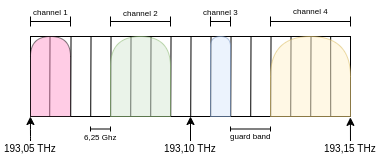
\includegraphics[scale=0.65]{flexigrid.png}}
	\caption{Flexigrid in EON}
	\label{eon_flexigrid}
\end{figure}

\section{Multicasting in WDM}

\subsection{Optimal multicast problem}
In \cite{wdm_biaochen} he proves that the problem of optimal wavelength assignment on a multicast tree is not NP-hard. Also proposed heuristic multicast routing algorithm. Authors discuss multicasting at WDM level, so very low physical layer.

In \cite{wdm_paira} she proposed a G-stream based approach to maximize resource utilization and minimize blocking probability with promising simulation results.

\subsection{IP-over-WDM networks}
In \cite{wdm_qiao} this is old study when technology was new, so good to compare expectation vs results

In \cite{wdm_zhang} this is same authors year later, so compare what they say with previous one

\section{Multicasting in EONs}
In \cite{eon_ghazijahani} An innovative RSA algorithm is proposed in the form of an optimization problem, that the cost function is the weighted sum of network cost with a proposed video quality cost

\section{Comparison of EON and WDM}
In \cite{wdm_eon_comparison} EON vs WDm comparison, very important. We observe consistent improvement in efficiency of flexible grid EONs over fixed-grid WDM networks


\begin{thebibliography}{00}
\bibitem{multicast_definition} K. Walkowiak, "Modeling and optimization of computer networks", \textit{PRINTPAP}, Wrocław University of Technology, 2011, pp. 66-67.
\bibitem{wdm_general} K. Walkowiak, "Modeling and optimization of computer networks", \textit{PRINTPAP}, Wrocław University of Technology, 2011, p. 10.
\bibitem{cwdm} "G.694.2: Spectral grids for WDM applications: CWDM wavelength grid", Telecommunications Standardization Sector of ITU, 2003.
\bibitem{dwdm} "G.694.1: Spectral grids for WDM applications: DWDM frequency grid", Telecommunications Standardization Sector of ITU, 2020.
\bibitem{eon_definition} B. Mikavica and A. Kostić-Ljubisavljević, "Security Issues of Cloud Migration and Optical Networking in Future Internet.", \textit{Cyber Security of Industrial Control Systems in the Future Internet Environment}, IGI Global, 2020, pp. 91-106.
\bibitem{eon_fs} E. Biernacka and A. Lasoń, "Elastic Optical Networks", Telekomunikacja i Techniki Informacyjne, 2013
%\bibitem{eon_orig} O. Gerstel, M. Jinno, A. Lord and S. Yoo, "Elastic Optical Networking: A New Dawn for the Optical Layer?", \textit{IEEE Communications Magazine} no. 50, 2012
\bibitem{wdm_qiao} C. Qiao, M. Jeong, A. Guha, X. Zhang and J. Wei, "WDM multicasting in IP over WDM networks," \textit{Proceedings. Seventh International Conference on Network Protocols}, 1999, pp. 89-96.
\bibitem{wdm_zhang} X. Zhang, J. Wei and C. Qiao, "On fundamental issues in IP over WDM multicast," \textit{Proceedings Eight International Conference on Computer Communications and Networks} (Cat. No.99EX370), 1999, pp. 84-90.
\bibitem{wdm_biaochen} B. Chen and J. Wang, "Efficient routing and wavelength assignment for multicast in WDM networks,", \textit{IEEE Journal on Selected Areas in Communications}, vol. 20, no. 1, pp. 97-109, 2002.
\bibitem{wdm_paira} S. Paira and U. Bhattacharya, "Efficient dynamic survivable multicasting in WDM mesh networks," 2018 10th International Conference on Communication Systems \& Networks (COMSNETS), 2018, pp. 525-527.
\bibitem{wdm_eon_comparison} A. Cai, Z. Fan, K. Xu, M. Zukerman and C. Chan, "Elastic versus WDM networks with dedicated multicast protection," \textit{Journal of Optical Communications and Networking}, vol. 9, no. 11, pp. 921-933, 2017.
\bibitem{eon_ghazijahani} H. Alizadeh Ghazijahani, H. Seyedarabi, J. Musevi Niya, and N. M. Cheung, "Optimized Routing and Spectrum Assignment for Video Communication over an Elastic Optical Network", 2019.
\end{thebibliography}
\end{document}
